\documentclass[12pt]{article}
\usepackage{tikz}
\usepackage[margin=1in]{geometry}
\usepackage{xcolor}
\usepackage{fontspec}

\usetikzlibrary{shapes,arrows,positioning,calc,fit}

\begin{document}

\begin{figure}[htbp]
\centering
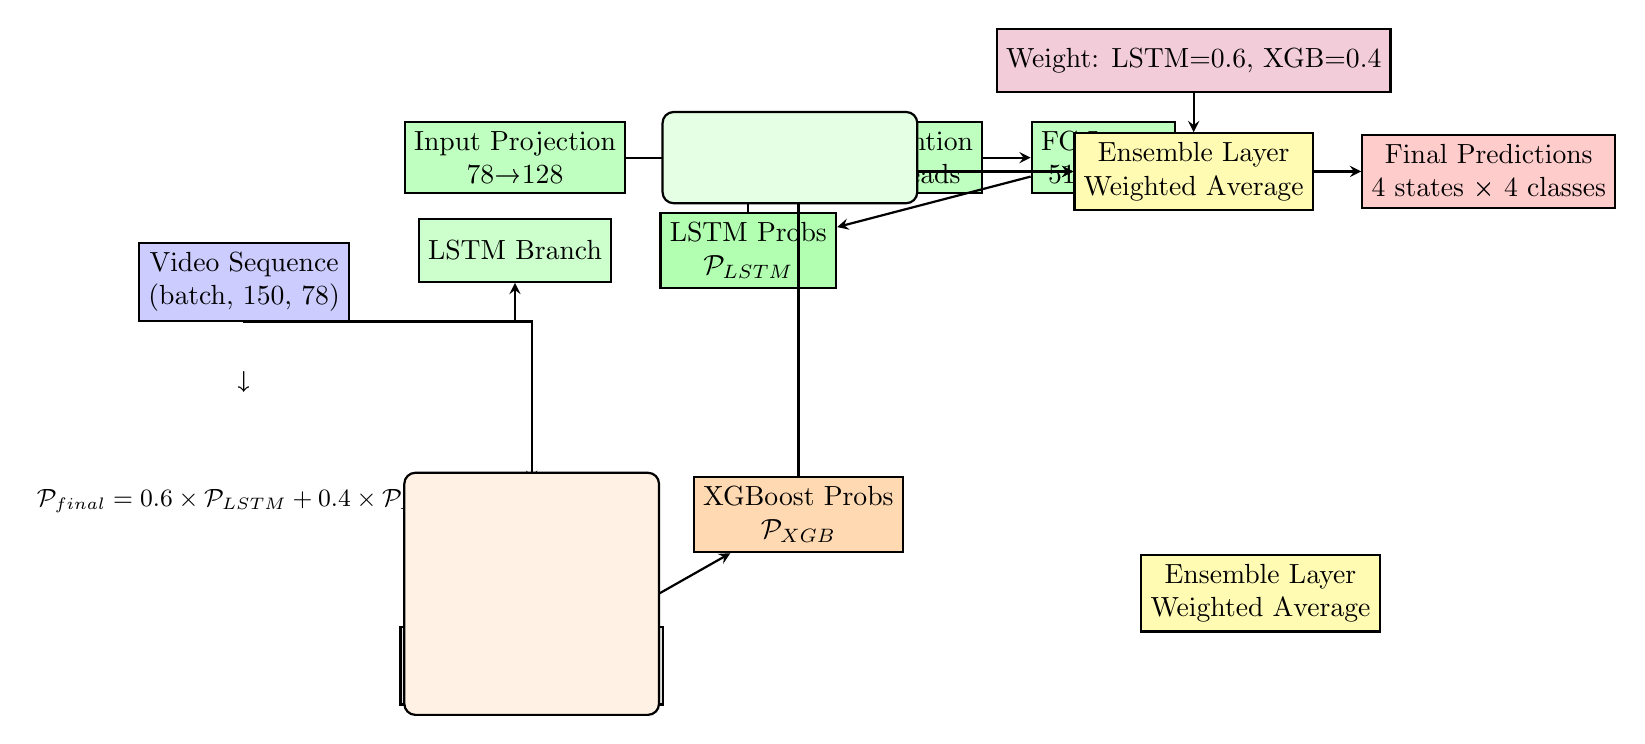
\begin{tikzpicture}[
    node distance=10mm and 6mm,
    box/.style={rectangle, draw, thick, align=center, minimum height=8mm},
    arrow/.style={->, thick, >=stealth},
    group/.style={draw, thick, rounded corners, fill=#1},
    label/.style={text width=3cm, align=center, font=\small\bfseries}
]

% Input
\node[box, fill=blue!20] (input) {Video Sequence \\ (batch, 150, 78)};

% Split into two branches
\node[below=0.5cm of input, font=\small] (split) {↓};

% LSTM Branch (top)
\node[box, fill=green!20, above right=1cm and 2cm of split] (lstm) {LSTM Branch};
\node[box, fill=green!30, right=of lstm] (lstm_out) {LSTM Probs \\ $\mathcal{P}_{LSTM}$};

% XGBoost Branch (bottom) 
\node[box, fill=orange!20, below right=1cm and 2cm of split] (xgb) {XGBoost Branch};
\node[box, fill=orange!30, right=of xgb] (xgb_out) {XGBoost Probs \\ $\mathcal{P}_{XGB}$};

% Feature Engineering
\node[box, fill=gray!20, below=1cm of xgb] (feat_eng) {Feature Engineering \\ (~2000 features)};

% Arrows from input
\draw[arrow] (input) -- ++(0,-0.5) -| (lstm);
\draw[arrow] (input) -- ++(0,-0.5) -| (xgb);
\draw[arrow] (xgb) -- (feat_eng);
\draw[arrow] (feat_eng) -- (xgb_out);

% LSTM arrows
\node[box, fill=green!25, above=0.3cm of lstm] (lstm1) {Input Projection \\ 78→128};
\node[box, fill=green!25, right=of lstm1] (lstm2) {BiLSTM \\ 2 layers};
\node[box, fill=green!25, right=of lstm2] (lstm3) {Attention \\ 8 heads};
\node[box, fill=green!25, right=of lstm3] (lstm4) {FC Layers \\ 512→128};

\draw[arrow] (lstm1) -- (lstm2);
\draw[arrow] (lstm2) -- (lstm3);
\draw[arrow] (lstm3) -- (lstm4);
\draw[arrow] (lstm4) -- (lstm_out);

% Ensemble Layer
\node[box, fill=yellow!30, right=3cm of lstm_out, yshift=1cm] (ens1) {Ensemble Layer \\ Weighted Average};
\node[box, fill=yellow!30, right=3cm of xgb_out, yshift=-1cm] (ens2) {Ensemble Layer \\ Weighted Average};

\draw[arrow] (lstm_out) |- (ens1);
\draw[arrow] (xgb_out) |- (ens1);

% Weights
\node[box, fill=purple!20, above=0.5cm of ens1] (weight) {Weight: LSTM=0.6, XGB=0.4};

% Final Output
\node[box, fill=red!20, right=of ens1] (final) {Final Predictions \\ 4 states × 4 classes};

\draw[arrow] (ens1) -- (final);
\draw[arrow] (weight) -- (ens1);

% Equation
\node[below=2cm of input, font=\small] (eq) {
$\mathcal{P}_{final} = 0.6 \times \mathcal{P}_{LSTM} + 0.4 \times \mathcal{P}_{XGB}$
};

% Legend/Groups
\node[group=green!10, fit=(lstm1) (lstm4), label={}] (lstm_group) {};
\node[group=orange!10, fit=(xgb) (feat_eng), label={}] (xgb_group) {};

\end{tikzpicture}
\caption{Ensemble Model Architecture: LSTM + XGBoost Hybrid Approach}
\end{figure}

\end{document}
